





The MeerKAT telescope consists of 64 receptors with 13.5\unit{m} diameter dishes, designed to achieve high sensitivity and imaging dynamic range, while providing an array and functionality to provide for a wide range of science. 
MeerKAT achieves a sensitivity of at least 220\unit{m2/K} at L-band (our designs indicate that we may achieve 300\unit{m2/K} in the L-band).\\
The high sensitivity requirement drives the design to multiple octave band single pixel feeds with cryogenic cooling. Three receivers cover the required operating band in the frequency ranges 0.58 - 1.015\unit{GHz}, 0.9 - 1.67\unit{GHz} and 8 - 14.5\unit{GHz}. 
The offset Gregorian dish configuration enhances sensitivity by providing high aperture efficiency and low spill-over temperature contribution. The offset Gregorian dish configuration also provides a clean optical path that can be designed to produce low overall sidelobe levels and azimuthal symmetry in the inner sidelobes to achieve high imaging dynamic range. \\
Low sidelobe levels also provide good rejection of unwanted radio frequency interference from satellites and terrestrial transmitters. The array configuration is designed with two components: a compact core containing 70 \% of the dishes, and an extended array
designed for high fidelity imaging performance over a range of resolutions from 6 arcsec to approximately 100 arcsec. \\
The overview of the MeerKAT telescope system illustrating major components and their functions  are shown in \textbf{Figure}~\ref{fig:image49}.

\section{Antenna Positioner} 
\begin{figure}[!thb]
	\centering
	%\includegraphicsdpi{100}{}{bur1.png}     
	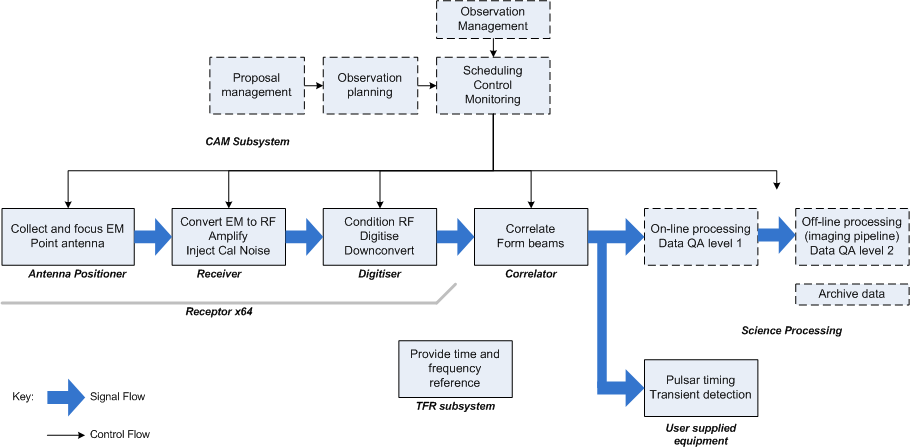
\includegraphics[scale=0.5]{Chapters/images/image49.png}
	
	%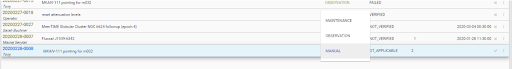
\includegraphics[resolution=100]{bur1.png}
	\caption{Overview of MeerKAT System}
	\label{fig:image49}
\end{figure}
The MeerKAT telescope array consists of 64 Receptors, each consisting of a steerable dish antenna, a set of radio receivers and a set of associated digitisers. The digitised radio signals are then transported over an array fibre network back to the central on-site data centre at the Karoo Array Processor Building (KAPB) where they undergo various stages of processing (correlation, beam forming and science processing) as shown in \textbf{Figure}~\ref{fig:image64}. The telescope array will be controlled and monitored from a number of remote locations, with the main control operations centre in Cape Town. The Receptor will be constituted by a Digitiser, an Antenna Positioner and a Receiver System.
\begin{figure}[H]
	\centering
	%\includegraphicsdpi{100}{}{bur1.png}     
	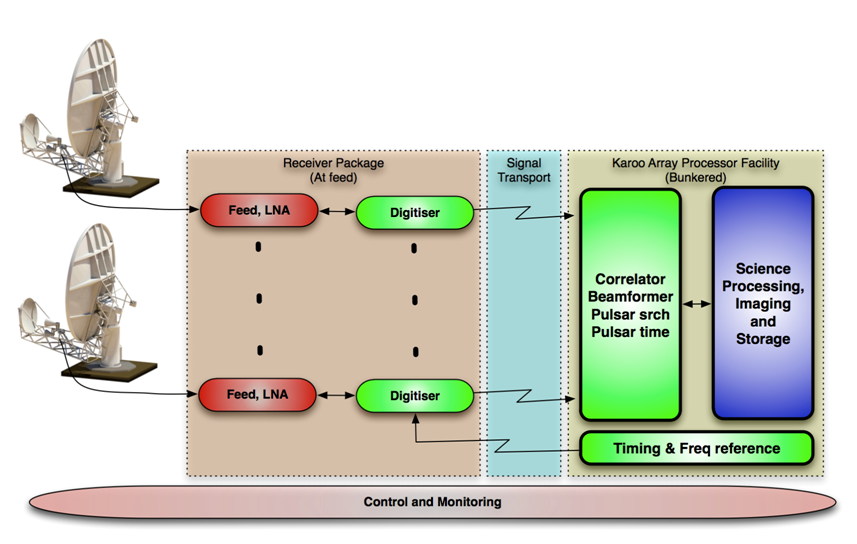
\includegraphics[scale=0.5]{Chapters/images/image64.png}
	
	%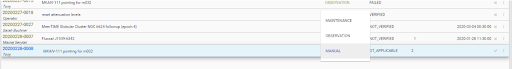
\includegraphics[resolution=100]{bur1.png}
	\caption{MeerKAT telescope signal path}
	\label{fig:image64}
\end{figure}
\section{Antenna Positioner}

The Antenna Positioner (AP)\cite{AP} main function is to intercept flux. This function will be provided by the Antenna Structure, Pointing Control System and Receiver Indexer major components of the AP. An offset Gregorian optical layout with a 13.5 m projected diameter aperture is chosen as it offers several advantages. The unblocked aperture of the offset design provides uncompromised optical performance and sensitivity, excellent imaging quality, and good rejection of unwanted radio frequency interference from satellites and terrestrial transmitters. This layout also provides space for a suite of receivers mounted on an indexer.
The Antenna Structure will be constituted by a dual reflector system mounted on an Elevation over Azimuth mount. The offset reflector will be part of the Reflector mounted on a Yoke. The Yoke provides the elevation and azimuth rotation to achieve pointing over the required observation range. Azimuth rotation is achieved by means of an Azimuth Drive and a geared Azimuth Bearing between the Yoke and the Pedestal. Pointing coordinates in the form of azimuth- (referenced from true North) and elevation values from the Telescope Control and Monitor subsystem (CAM) are received and interpreted by the Position
Controller, and executed by the Elevation and Azimuth Drives of the Pointing Control System. The Antenna Positioner provides monitoring information to the Telescope and implements a standardised monitor and control interface (KATCP) over TCP/IP.
The 4 receivers of the Receiver System are mounted on the Receiver Indexer of the Antenna Positioner[TBD].

\section{Receiver System}
The MeerKAT receiver system\cite{RSC} consists of the following major components: a UHF-band receiver, an L-band receiver, a vacuum pump station, a helium compressor and a receiver system controller (RSC). The receivers and vacuum pump station are mounted onto the receiver indexer, the helium compressor is mounted onto the yoke and the RSC slots into the 19” rack in the shielded drive compartment of the antenna pedestal. The receiver system is designed to operate with 4 receivers and thus makes provision for 2 more receivers
to be added in the future. The receivers use Gifford-McMahon (GM) cryogenic cooling which significantly exceeds the current sensitivity specification[TBD].
\section{Digitiser System}
The main function of the Digitiser\cite{DIG} is to digitise the analogue RF signal provided by the receivers. RF signals from both polarisations of each feed enter the appropriate Digitiser and get conditioned via an analogue RF conditioning section before entering the ADC. 
The RF conditioning section filters and amplifies the signal before entering the ADC. Filtering is performed in such a manner that Digitiser efficiency as well as out-of band suppression requirements are achieved. 
Further functionality of the RF conditioning section is to provide adjustable gain to improve telescope operational dynamic range, power detection of incoming and pre-ADC RF levels and potential bi-phase modulation to improve RF channel isolation. All analogue electronics preceding the ADC is potentially thermally controlled to the temperature that results in the best phase and amplitude stability of the RF signal. An ultra high speed ADC samples the conditioned RF based on a sample clock that is provided by the TFR subsystem.
High speed optical interfaces between the ADC and the D engine ensure that RFI generated by these assemblies do not degrade the Digitiser RFI performance.
The D engine receives the digitised data from the ADC and depending on what Nyquist zone is being sampled, down-convert the entire band to baseband frequencies using a DDC with programmable LO.  The down-converted signal is packetized and transported to the Correlator data switch via Ethernet fibre optic links. All data products are time stamped with the Digitiser local time which is derived from the 1 pulse per second (1PPS) signal provided by the TFR via analogue fibre. Control and Monitoring of the Digitiser as well as data transport from the Digitiser to the Correlator is performed on the same optical Ethernet interface [TBD].
\section{ CAM System}
The CAM subsystem\cite{CAM} is responsible for Control and Monitoring of the MeerKAT telescope and presentation of the CAM user interfaces for operators, engineers and science users.
The CAM subsystem shall monitor all monitoring points for health, state and alarms, archive history of all monitoring points and allow easy interrogation of the monitoring archive.
The CAM subsystem shall provide a Proposal Management Tool that will support the proposal process from application submission through to final approval, 
as well as provide mechanisms required by the Observation Planning Tool (responsibility of the Science Processing Team) [1]. 
The Observation Planning Tool (OPT) will support the observer in preparing the program and scheduling blocks for an approved proposal and may need mechanisms from CAM e.g. to simulate or dry-run observation execution.
The CAM subsystem shall control the telescope during observations including scheduling, configuring and controlling other subsystems, monitoring execution of programs, 
noting the data products produced and preparing an observation report on completion of each program.
\section{ Correlator BeamFormer}
The Correlator-Beamformer (CBF)\cite{CBF} is configurable for a range of data products to support all
the required types of observations. This includes spectral line and continuum imaging, pulsar
timing, tied-array beamforming and various transient search functions. It uses a packetized
architecture comprising switches and reconfigurable modular processing elements, which
makes it flexible, upgradeable and scalable.
\section{ Science Processor}
The Science Processor (SP)\cite{SP} is a subsystem of the MeerKAT telescope whose primary role is the
production of science quality output from the raw data provided by the Correlator-Beamformer subsystem. 
The SP includes both visibility and time-domain processing capabilities, along with an
extensive archiving component, and a variety of user interfaces, including the primary point
of interaction with the science users in the form of the Observation Planning Tool.
The SP can be regarded as the terminal system of the telescope, with downstream
interactions leaving the boundaries of the telescope system itself.
\section{Time and Frequency Reference System}
The Time and Frequency Reference (TFR)\cite{TFR} is an essential subsystem of the MeerKAT, in providing absolute traceable time to the system using atomic clocks. This is necessary in nearly all the telescope functions.
Frequency directly impacts the quality of data and time itself forms part of the telescopes signal data products, as this measurement together with other data, enables specific science including precision astrometry. 
This specific requirement specification document largely focuses on a correct implementation for the L-band, but equipment specification for equipment clocks is done, 
so as not to limit adaptability to other bands including S-band and X-band. Furthermore the pulse per second specifications is applicable to any band. Certain specifications are however left open for the S and L-bands.
The function of the TFR subsystem is to provide and distribute accurate time to the Telescope system. It is also expected to provide both PPS and PTP to be used by other subsystems of the telescope.
